\chapter{Introducción}
%%%%%%%%%%%%%%%%%%%%%%%%%%%%%%%%55%%%%%%%%%%%%%%%%%%%%%%%%%%%%%%%%%%%%%%%%%%%%%%%%%%%%%%%%%%%%%%%%%%%%%%%%%%%%%%%%%%%%%%%%%%%%%%%%%
% requerimientos,Hacer como una sinopsis.
%%%%%%%%%%%%%%%%%%%%%%%%%%%%%%%%%%%%%%%%%%%%%%%%%%%%%%%%%%%%%%%%%%%%%%%%%%%%%%%%%%%%%%%%%%%%%%%%%%%%%%%%%%%%%%%%%%%%%%%%%%%%%%%%%%%

Este documento presenta las tareas realizadas en el marco del proyecto de fin de carrera ``Análisis de Video en Biomecánica'' realizado en la Facultad de Ingeniería, Universidad de la República (UdelaR). A continuación, se hace una introducción a la problemática encontrada, en función de la cual se plantea el objetivo del proyecto y una breve descripción de las soluciones actualmente disponibles.
\vspace{5 mm}

Especialistas de distintos ámbitos académicos o profesionales se encuentran habitualmente en la necesidad de realizar estudios del movimiento del cuerpo humano. Esta tarea implica registrar la posición de miembros o articulaciones en el espacio y su correspondiente evolución en el tiempo.
\\ 

Algunos ejemplos correspondientes a distintas áreas que ilustran estas necesidades son:

\begin{itemize}
\item A \emph{nivel asistencial}, en el área de \emph{fisioterapia}. Para realizar un seguimiento de la evolución de un paciente resulta importante en muchos casos conocer en detalle el movimiento, posición, etc. de la articulación o miembro afectado para llevar un control del mismo durante la rehabilitación y así poder determinar con mayor exactitud el estado y la evolución del paciente.
\item \emph{Investigación académica en biomecánica}. Diversos proyectos se llevan a cabo en las universidades sobre esta temática, por ejemplo, en la Facultad de Ingeniería de la Udelar  se realizó el estudio comparativo de la patada delfín y la patada “crawl” respecto al nado de los peces por ondulación, tratando de explicar cómo la misma puede ser propulsiva. Para ello se analizaron videos de nadadores olímpicos mediante los cuales se obtuvo una secuencia temporal de las posiciones de diferentes partes del cuerpo durante varios ciclos de patada\footnote{\textcolor{blue}{\scriptsize{\underline{\url{ http://www.fing.edu.uy/ingenieriademuestra2011/proyectos/proyectos-del-instituto-de-f\%C3\%ADsica}}}}. Accedido 20-12-14}.
\item \emph{Medidas de performance en el deporte de alto nivel}. Cuando se habla de entrenamiento deportivo se hace referencia tanto a la mejora del rendimiento del atleta como a la optimización de las capacidades en función del deporte en el que se desempeña. La técnica deportiva está relacionada directamente con la optimización de estas capacidades por lo que una buena técnica permite el mejor aprovechamiento de las posibilidades físicas del atleta garantizando mejores resultados. Las mejores soluciones para la optimización de la técnica de un deportista consisten en el análisis de videos donde se puede estudiar en detalle cada uno de los movimientos del  mismo.
\item \emph{Animación 3D}. Probablemente el más conocido de estos ejemplos, tanto en el diseño de videojuegos como en películas, programas de televisión o comerciales, muchas veces se requiere capturar el movimiento de un actor para interpretar un personaje ficticio y que sus movimientos parezcan lo más natural posible. En el medio local existen empresas que se dedican a esto, tales como Mopix \cite{mopix}.
\end{itemize}

En este contexto, el análisis de video  es  una  herramienta  fundamental para la recolección y estudio de datos. El seguimiento de puntos de referencia se utiliza para el cálculo de posición y otras variables asociadas como son la velocidad, la aceleración y por ende desplazamientos. Trabajar con video permite además estudiar secuencialmente situaciones estáticas en el tiempo. El seguimiento de dichos puntos resultaría tedioso si se hiciera manualmente por lo que resulta necesario contar con una herramienta que realice esta tarea automáticamente.
\\ 

A raíz de esto, se crean los \emph{sistemas de captura de movimiento}, que se definen como un conjunto de dispositivos y software que a partir de la grabación del movimiento de una persona (o cualquier otra cosa), es capaz de trasladar dicho movimiento a un modelo digital para diferentes fines.
\\ 

Los ejemplos mencionados anteriormente definen distintos casos de uso con características disímiles, de manera que la búsqueda de una solución única que abarque las necesidades particulares de todos ellos resulta compleja. Por ejemplo, en el ámbito deportivo la velocidad del movimiento es una variable importante a tener en cuenta para desarrollar una solución, de esta variable depende la elección tanto del sistema de adquisición como de los algoritmos más eficaces para el registro del movimiento.  De igual manera definir la portabilidad del sistema depende de si la actividad a relevar es en condiciones de laboratorio controladas o al aire libre, debido a la protección y transporte de equipos o las variaciones en las condiciones de iluminación, ruido, etc..
\\ 

Al  día  de  hoy, las  soluciones  de  software  disponibles que  podrían  asistir al especialista en su tarea, son mayormente comerciales. Las pocas alternativas de código abierto, carecen de las características necesarias para el especialista o están enfocadas hacia otras áreas de aplicación. Contar con este tipo de herramientas es fundamental para las necesidades de los equipos de profesionales, cuya alternativa son productos comerciales de alto costo.
\\ 

En virtud de estas necesidades, este proyecto busca {relevar y caracterizar los distintos casos de uso para un sistema de captura de movimiento, seleccionar uno que sea representativo y suficientemente general para poder realizar una aplicación básica y funcional de código abierto de análisis de video, que proporcione solución a las necesidades que se describieron ya sea utilizando como base algún  proyecto  de  software  libre  existente, o en su defecto, desarrollando un prototipo de software básico completo que abarque el problema en forma general, para luego estudiar extender la aplicación hacia otros casos de uso}.
\\ 

Es importante resaltar la importancia de tener una primera versión del sistema de principio a fin, con todas las etapas implementadas, de forma tal de abarcar todos los procesos que la captura de movimiento implica.  Esto tiene como ventaja que se tendrá un panorama general del estado del arte de cada etapa del sistema, y 
sentará las bases para que proyectos futuros puedan optimizar individualmente dichas etapas acorde a las necesidades del cliente.
\\ 

Los requerimientos para la implementación de este sistema provienen de investigadores del Departamento de Biofísica de la Facultad de Medicina de la Udelar, el foco del proyecto es la investigación no asistencial pero también puede utilizarse para fines asistenciales, particularmente el estudio del movimiento de las personas.
\\ 

De acuerdo a lo planteado por el cliente y a las hipótesis que se establecieron en conjunto, se plantean los siguientes supuestos relativos a la apariencia del laboratorio:
\begin{itemize}
\item Las capturas de movimiento del paciente se realizan en un ambiente controlado:\vspace{-0.2cm}
	\begin{itemize}
		 \item La iluminación es la adecuada para realizar las  capturas correctamente.
		 \item El fondo sobre el que se hacen las capturas es estático, de color oscuro y opaco.		 
		 \item Se utiliza cámaras convencionales y la ubicación de las cámaras así como sus parámetros de interés son conocidos.
	\end{itemize}
	\vspace{-0.2cm}
\item La vestimenta que utiliza el paciente es oscura, opaca y lo más ajustada al cuerpo como sea posible.\vspace{-0.1cm}
\item Los marcadores a detectar son esferas blancas colocadas convenientemente sobre el cuerpo del paciente.
\end{itemize}

En cuanto al movimiento se asume que:
\begin{itemize}
\item El paciente permanece dentro del área de captura.\vspace{-0.1cm}
\item Existe oclusión de marcadores en vistas dadas.\vspace{-0.1cm}
\item Las cámaras se mantienen fijas.
\end{itemize}

Por otro lado, como se muestra en la Figura \ref{abuela2} se requiere que la salida del sistema sea la posición en el espacio 3D de los marcadores, ubicados en el cuerpo del paciente, en cada instante de la captura, con la correcta identificación de dichos marcadores en cada cuadro. A estos requerimientos, se le suman otros de carácter académico, como la importancia de tener una base de datos con un cierto número de secuencias y una método de evaluación de performance establecido. Estos dos aspectos toman gran relevancia en etapas futuras, de ampliación de este proyecto, ya que al realizar pruebas  de nuevas implementaciones sobre los mismos datos y evaluar los resultados con iguales métricas se tiene un punto de referencia sobre el cual evaluar posibles mejoras del sistema.
\\ 

En resumen, el sistema creado pretende bajo ciertas condiciones controladas, obtener las coordenadas espaciales de un número de puntos de interés sobre una paciente. Una de las formas de obtener esto, y la estudiada en este trabajo, es colocar al sujeto con traje negro con marcadores en un ambiente con iluminación adecuada, filmar con varias cámaras a lo largo del tiempo, adquirir esta información en la computadora y mediante un posterior procesamiento obtener la posición 3D de cada uno de los puntos de interés (los marcadores) a lo largo de toda la secuencia.

\begin{figure}[H]
\begin{center}
\includegraphics[scale=0.4]{img/Sistema_completo/diagrama_abuelas_2.jpg}
\end{center}
\caption{Posición de los marcadores a lo largo del tiempo.}
\label{abuela2}
\end{figure}

La aplicación recibe como entrada imágenes de video provenientes de varias cámaras, las cuales capturan el movimiento de una persona desde distintos ángulos. Se implementan métodos que permiten obtener información sobre las cámaras y su disposición en el espacio mediante la calibración. Con esta información y a partir de las imágenes obtenidas se detectan distintos puntos de referencia del cuerpo según el estudio particular que se desee realizar. Posteriormente, a partir de la información de las múltiples cámaras se reconstruye la posición 3D de los puntos en cada cuadro, para luego efectuar la identificación de trayectorias de los puntos de interés a lo largo de la secuencia, ver Figura \ref{abuela1}. A partir del procesamiento de la posición 3D de los puntos se obtendrán otros datos estadísticos de interés para el usuario.\\

\begin{figure}[ht!]
\begin{center}
\includegraphics[scale=0.4]{img/Sistema_completo/diagrama_abuelas_1.jpg}
\end{center}
\caption{Funcionamiento de un sistema de captura de movimiento.}
\label{abuela1}
\end{figure}


%SINOPSIS
El proyecto se inicia con investigación y revisión bibliográfica sobre la temática, buscando diseños provenientes de sistemas de captura de movimiento ya implementados, así como  detalles sobre la implementación parcial o total de cada funcionalidad de interés. 
\\ 

Rápidamente se procuró obtener una base de datos con secuencias, ya sean reales o sintéticas, sobre los cuales implementar la aplicación y sus distintos bloques. Si bien esta búsqueda no aportó los resultados esperados,
%no obtuvo buenos resultados %ME QUERES MATAR ANDREI!!!!
 debido a que no se encontraron bases de datos acorde a las necesidades del proyecto, se implementa un prototipo de base de datos sintética con un número reducido de secuencias como alternativa tomando algunos conceptos encontrados en dicho relevamiento, generando una base flexible, de fácil expansión y con potencial para futuros estudios.\\ 

 Luego de analizar la bibliografía y definir la metodología, se opta por implementar el sistema con los 4 bloques principales mostrados en la Figura \ref{bloquesSistintro}. 

 \begin{figure}[H]
\begin{center}
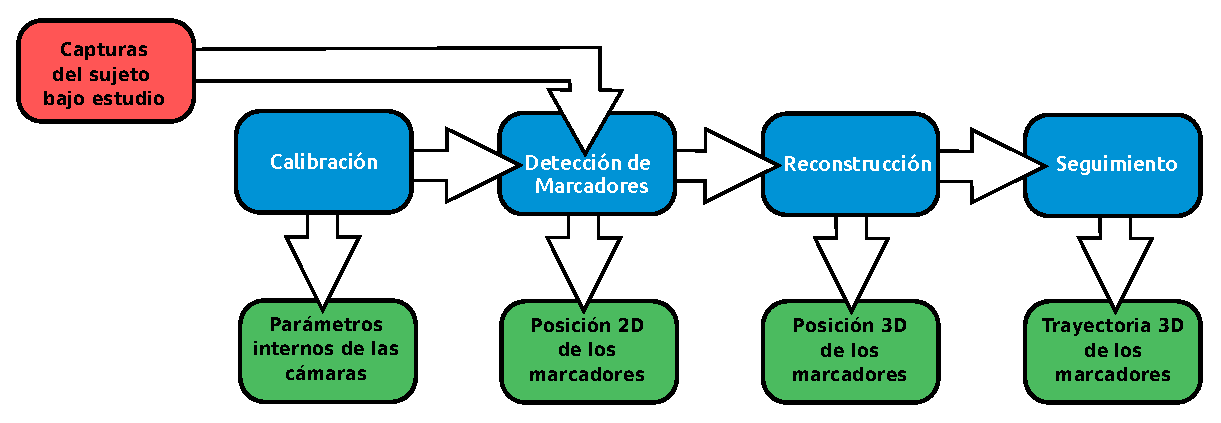
\includegraphics[scale=0.7]{img/Sistema_completo/Diagrama_de_bloques.eps}
\end{center}
\caption{Diagrama de bloques del sistema a implementar.}
\label{bloquesSistintro}
\end{figure}

Cada uno de estos bloques cumple un objetivo definido:
\begin{itemize}
\item El bloque de \emph{calibración}, es el encargado de obtener los parámetros internos y externos de las múltiples cámaras utilizadas en la captura, permitiendo establecer la relación entre el espacio ambiente y la imagen sobre cada cámara. Una vez que se disponen el número y posición de las cámaras para efectuar la captura de movimiento, este bloque releva por única vez la información previa necesaria para realizar una correcta reconstrucción de los puntos.
\item El bloque \emph{detección de marcadores}, identifica los marcadores en las imágenes obteniendo la posición 2D de cada uno de ellos a lo largo de la secuencia de captura en cada cámara (ver Figura \ref{peladocirculosintrointro}).
\item Con información de posición 2D proveniente de la detección de marcadores en múltiples vistas, y los parámetros relevados en calibración, el bloque de \emph{reconstrucción} (ver Figura \ref{peladoewconstruidointro}) se encarga de obtener la posición 3D de cada marcador.
\item Por último, el bloque de \emph{seguimiento} (ver Figura \ref{peladoetrackingintro})
(o ``tracking'') relaciona cada marcador en determinado cuadro de la secuencia con los que le siguen en el resto de los cuadros, obteniendo así la trayectoria de cada marcador a lo largo del tiempo.
\end{itemize}

Cabe destacar que estos bloques se implementaron de manera independiente, con una interfaz claramente definida, de manera  de poder realizar modificaciones sobre uno de ellos sin afectar el funcionamiento de los otros. Este aspecto cobra relevancia en etapas futuras, donde bajo la necesidad de optimizar algún bloque en particular o agregar alguna nueva característica que permita procesar datos provenientes de nuevos casos de uso, se deba modificar el sistema. De no presentar esta particularidad, la modificación de un bloque podría afectar el funcionamiento del sistema completo, requiriendo una posible re-ingeniería de la estructura.

\begin{figure}[ht!]
        \centering
        \hspace{1.3 cm}
        \subfloat[Captura original]{\includegraphics[scale=0.4]{img/peladoFondoAzul.png} %\label{peladoOriginalintrointro}
        }\hspace{2.2 cm}
        \subfloat[Detección de marcadores]{\includegraphics[scale=0.4]{img/peladoFondoAzul_circulos.png}\label{peladocirculosintrointro}}

        \subfloat[Recontrucción 3D]{\includegraphics[scale=0.15]{img/Reconstruccion/reconstruccion1.png}\label{peladoewconstruidointro}}
    	\subfloat[Seguimiento]{\includegraphics[scale=0.24]{img/Tracking/track1.png}\label{peladoetrackingintro}}  
  \caption{Salidas de los bloques principales del sistema.}
      \label{ejemplotutiintro}
\end{figure}

Por otro lado, fue elaborada una interfaz gráfica básica de forma tal de facilitar la ejecución del software para los usuarios sin tener que trabajar directamente con el código.
\\ 

A continuación se presenta una breve revisión del estado del arte de los sistemas de captura de movimiento disponibles. Una descripción más detallada y más técnica se realizará en la Sección \ref{invBiblio}, luego se define el objetivo del proyecto y se comenta la estructura de la documentación.

\section{Estado del arte}
%%%%%%%%%%%%%%%%%%%%%%%%%%%%%%%%%%%%%%%%%%%%%%%%%%%%%%%%%%%%%%%%%%%%%%%%%%%%%%%%%%%%%%%%%%%%%%%%%%%%%%%%%%%%%%%%%%%%%%%%%%%%%%%%%%%5
%qué opciones tengo para hacerlo? por qué hay estas opciones? para qué se usan?
%%%%%%%%%%%%%%%%%%%%%%%%%%%%%%%%%%%%%%%%%%%%%%%%%%%%%%%%%%%%%%%%%%%%%%%%%%%%%%%%%%%%%%%%%%%%%%%%%%%%%%%%%%%%%%%%%%%%%%%%%%%%%%%%%%%

Al día de hoy existen varios sistemas de captura de movimiento, sin embargo los mas usados debido a su buena performance y soporte presentan altos costos de licenciamiento. 
\\ 

Como se mencionó anteriormente, los más populares en la actualidad son los que se utilizan en la industria del cine o del diseño de videojuegos. En este contexto, se almacenan las acciones de actores humanos y se usa esta información para animar modelos digitales de personajes en animación 3D.
\\ 

Algunos ejemplos de sistemas de captura de movimiento bajo licencia son:

\begin{itemize}
\item \emph{Vicon} \cite{vicon}. Es una empresa que vende sistemas de captura de movimiento, tanto software como hardware. Sus sistemas son muy conocidos y fuertemente utilizados en estudios clínicos y biomecánicos alrededor del mundo, así como para otras investigaciones científicas. En particular, este sistema está siendo utilizado en el Departamento de Fisiatría y Rehabilitación del Hospital de Clínicas. Presenta como ventajas frente a otros sistemas la velocidad con que realiza el procesamiento de los datos y la calidad de las cámaras para realizar las capturas. La gran desventaja que posee es el alto costo de sus equipamientos, bastante privativo en algunos ámbitos.
\item \emph{Qualisys} \cite{qualisys}. Junto con Vicon son los dos sistemas de captura de movimiento más utilizados en el ámbito de la investigación científica. Presenta como ventajas frente al anterior la utilización del modelo AIM\footnote{Automatic Identification of Markers}, un identificador de marcadores que ``aprende'' de cada secuencia procesada ahorrando mucho tiempo y trabajo en identificar marcadores. Además presenta una interfaz de usuario más amigable y requiere menos tiempo de capacitación para su uso.
\item \emph{OptiTrack} \cite{optitrack}. Es de los sistemas comerciales de menor costo, cerca de la cuarta parte de lo que cuesta un sistema Vicon. Otra de sus ventajas es que brinda acceso de bajo nivel a través de un conjunto de  SDK's y API's tanto para el hardware como para los datos obtenidos, permitiendo manipular los mismos y procesarlos de la manera deseada por fuera de las aplicaciones que originalmente provee. 
\item \emph{Massive} \cite{massive}. Es un software destinado a producir efectos especiales para cinematografía, programas televisivos y videojuegos entre otras cosas. El software implementa la captura de movimiento y cuenta con varios productos para generar distintos tipos de efectos y animaciones. Fue originalmente diseñado par utilizar en la trilogía de El Señor De Los Anillos de Peter Jackson y desde entonces se ha convertido en uno de los mejores software para realizar efectos visuales de muchedumbres y animación de personajes autónomos.
\item \emph{Motion Analysis} \cite{motion_analysis}. es el mayor fabricante mundial de sistemas de instrumentación óptica de alto rendimiento que permite testear y medir el movimiento de los objetos. Mantiene y comercializa el software con sus sistemas de hardware. Sus sistemas evalúan el movimiento en distintas aplicaciones: producción de animación, análisis de movimiento, y en el ámbito industrial. Posee un gran número de aplicaciones de pos-producción.

\item \emph{PhaseSpace} \cite{phasespace}. Posee un sistema de captura patentado basado en marcadores leds, de alta resolución temporal y espacial. Todo el sistema se compone de sólo unos pocos elementos robustos y portátiles. Sus aplicaciones funcionan tanto en entornos Linux como Windows. Ha desarrollado soluciones de captura de movimiento para la investigación, la industria y las comunidades de las artes gráficas, también para estar al alcance de las pequeñas empresas, universidades y particulares.
\end{itemize}

Los sistemas anteriores, y la mayoría de los sistemas modernos que efectúan capturas de movimiento, utilizan sensores infrarrojos o LEDs para efectuar el seguimiento de puntos. Los segundos facilitan la etapa de detección de marcadores en cada cámara, mientras que los primeros no tienen una etapa de detección en cada vista ni reconstrucción ya que los mismos ofrecen la información de posición directamente.
\\ 

La gran desventaja de los sistemas anteriores es su alto costo. A modo de ejemplo, un sistema Vicon de 10 cámaras tiene un valor que ronda los U\$S\;70.000 \footnote{Este precio depende fuertemente del tipo de cámara que se utilice, los precios de las mismas se encuentran a partir de los U\$S\;3.000 por unidad.}.
\\ 


Por otro lado, también existen programas de captura de movimiento de código libre, un ejemplo de ello es el programa Kinovea \cite{kinovea}. Enfocado principalmente en el ámbito deportivo, permite analizar y mejorar la técnica de los atletas a través del procesamiento de secuencias de video. Posee algunas características interesantes como la posibilidad de efectuar medición de distancias, ángulos y tiempos manualmente, así como la utilización de seguimiento semi-automático de puntos en tiempo real para obtener su trayectoria. La gran desventaja que presenta frente a otros sistemas es que efectúa únicamente análisis sobre dos dimensiones y con una sola cámara.\\

Otra alternativa sobre la que se investigó es DVIDEOW \cite{figueroa2003flexible}. Este software presenta varios conceptos teóricos como primer acercamiento al problema, pero la implementación presenta pérdidas de marcadores que requieren correcciones constantes. Además, no se tiene una actualización del mismo desde el 2009, desde esa fecha a la actualidad solamente se encontraron trabajos que lo presentan como fundamento teórico.

\section{Objetivo del proyecto}

Desarrollar un prototipo de software básico pero completo que permita tener un sistema de captura de movimiento de punta a punta.\\

Diseñar una base de datos que permita organizar la información recabada en las capturas para un posterior procesamiento.\\

Definir un protocolo para la adquisición de secuencias de movimiento basado en un sistema de captura óptico.\\

Contar con medidas de performance que permita evaluar y comparar los algoritmos desarrollados. 




\section{Estructura de la documentación}

En este capitulo se presentó el objetivo general del proyecto y un breve estado del arte de la temática que será desarrollado profundamente en el Capítulo~\ref{invBiblio}, junto a un planteo en la Figura~\ref{bloquesSistintro} de los bloques que se estudiarán a lo largo del proyecto. 
\\

El Capítulo~\ref{section_base_de_datos} presentará un estudio de bases de datos disponibles y como fueron generadas capturas experimentales propias sobre las cuales trabajar. Luego el Capítulo~\ref{sec:implementacion_bloques_sistema} presentará detalles sobre el procedimiento de la Figura~\ref{bloquesSistintro} a partir de los datos experimentales generados. 
\\

En los capítulos siguientes se presentará como fue estudiado e implementado cada bloque: Segmentación y Filtrado en el Capítulo~\ref{deteccionMarcadoresSec} para la detección de la posición de los marcadores en cada video, Calibración en el Capítulo~\ref{calibracion} donde se mostrará como se genera la información del espacio de captura necesaria para luego en el Capítulo~\ref{reconstruccion} sobre Reconstrucción, mostrar como se combina la información de los bloques anteriores para calcular la posición en el espacio de los marcadores. 
\\

Posteriormente, el Capítulo~\ref{seguimiento} sobre Seguimiento propone un método de identificación de marcadores reconstruidos. 
\\

Finalmente se presenta cómo fue evaluado cada bloque y múltiples pruebas sobre el sistema completo en el Capítulo~\ref{evaluacion} para luego presentar las conclusiones en el Capítulo~\ref{conclusiones}.


 
  


%Dada las características de este proyecto otro antecedente relevante a tener en cuenta en el área, es el de un grupo de investigadores del Hospital de Clínicas que junto al grupo de Tratamiento de Imágenes de la Facultad de Ingeniería han estudiado previamente la marcha de las personas a los efectos de reconocer en ellas patrones de movimiento. Dicho proyecto recibe el nombre “Cíclope”.